\section{Resultados}

En esta sección se van a presentar los resultados obtenidos tras realizar el estudio del fenotipo Disgrafía.

\subsection{Grafo bipartito}

Se ha observado, gracias al grafo proyectado de genes, que la disgrafía se relaciona con todos los 51 del archivo del que se obtuvo el grafo y (por medio de dichos genes) a 1357 términos HPO distintos. Como resultados del grafo bipartito se ha obtenido una tabla con las relaciones de cada uno de los HPOs acompañados por su nombre e identificador, ordenados según el número de genes que relacionen ese HPO con el de la disgrafía. En la tabla \ref{tab:dysgraphia-relaciones} se visualiza los HPO más realcionados con Disgrafía.

\begin{table}[h]
	\caption{HPO más relacionados con dysgraphia.}
	\label{tab:dysgraphia-relaciones}
	\centering
	\begin{tabular}{|c|c|c|}
		\hline
		\textbf{id HPO} & \textbf{Nombre} & \textbf{nº de genes} \\
		\hline
		HP:0010526 & Dysgraphia & 51 \\
		HP:0001288 & Gait disturbance & 45 \\
		HP:0000716 & Depression & 44 \\
		HP:0001260 & Dysarthria & 42 \\
		HP:0000739 & Anxiety & 42 \\
		HP:0002167 & Abnormality of speech or vocalization & 40 \\
		HP:0002017 & Nausea and vomiting & 38 \\
		HP:0001249 & Intellectual disability & 36 \\
		HP:0000505 & Visual impairment & 35 \\
		HP:0007018 & Attention deficit hyperactivity disorder & 35 \\
		\hline
	\end{tabular}

\end{table}


\subsection{Red de genes asociados}

Después de descargar la red de genes asociados a la Disgrafía de la HPO, observamos que contenía 51 genes. Posteriormente, obtuvimos la red de esos genes utilizando la base de datos STRING-DB, la cual se puede observar en la imagen \ref{fig:genesAsociados}.

\begin{figure}[h!]
	\centering
	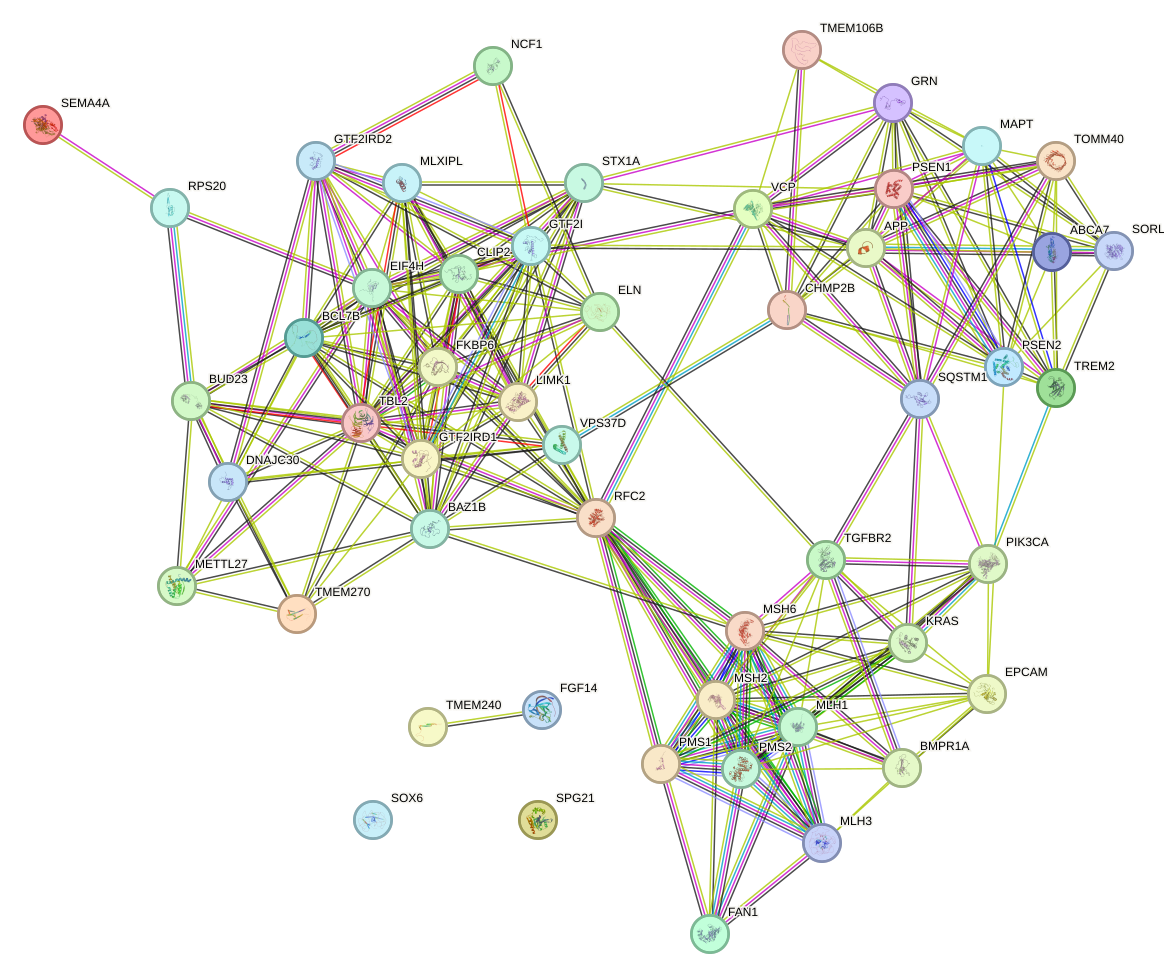
\includegraphics[width=0.7\textwidth]{figures/stringdb_51_genes.png}
	\caption{Red de genes asociados}
	\label{fig:genesAsociados}
\end{figure}

Se aplicó el algoritmo Diamond para propagar la red de genes y descubrir potenciales genes adicionales relacionados con la Disgrafía. El resultado de este proceso se encuentra en el archivo "propaged\_genes.txt", que contiene un listado con 200 genes. Utilizando estos genes, se creó una red mediante la librería de String. La cabecera del archivo que contiene la red se puede visualizar en la tabla \ref{tabla:resultDiamond} (se han omitido algunas columnas del archivo para mejor visualización).

\begin{table}[h]
	\centering
	\caption{Red de genes con los resultados de Diamond}
	\label{tabla:resultDiamond}
	\begin{tabular}{|c|c|c|c|c|c|}
		\hline
		stringId\_A & stringId\_B & preferredName\_A & preferredName\_B & score \\
		\hline
		9606.ENSP00000013807 & 9606.ENSP00000265433 & ERCC1 & NBN & 0.7 \\
		9606.ENSP00000013807 & 9606.ENSP00000347232 & ERCC1 & BLM & 0.701 \\
		9606.ENSP00000013807 & 9606.ENSP00000494957 & ERCC1 & UBE2T & 0.702 \\
		9606.ENSP00000013807 & 9606.ENSP00000229769 & ERCC1 & FANCE & 0.71 \\
		\hline
	\end{tabular}
\end{table}

Cada fila de esta red contiene información sobre la interacción de dos proteínas. Las cuatro primeras columnas incluyen los identificadores de los dos genes que están interactuando (tanto el StringId como el nombre). La cuarta columna (\textit{score}) es la puntuación combinada, la cual ya se mencionó en la sección \ref{section:redProteinas}.


\subsection{Detección de comunidades}

Se realizó un análisis de detección de comunidades en la red ampliada de genes. El algoritmo greedy\_modularity\_communities de NetworkX se empleó para identificar conjuntos de genes más densamente conectados entre sí. Los resultados de este análisis se presentan en la imagen \ref{fig:comunidades}.

\begin{figure}[h!]
	\centering
	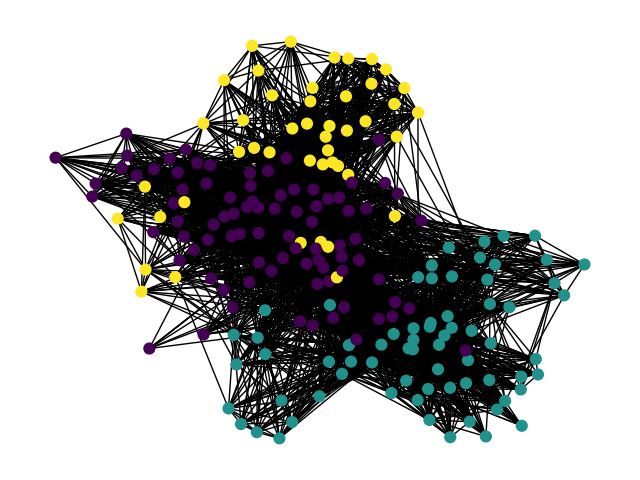
\includegraphics[width=0.7\textwidth]{../results/graph_communities.png}
	\caption{Comunidades de la red de genes}
	\label{fig:comunidades}
\end{figure}

Este algoritmo ha detectado tres comunidades. Cada color de la imagen \ref{fig:comunidades} representa una comunidad distinta.

\subsection{Enriquecimiento}

Se llevó a cabo un análisis de enriquecimiento funcional para identificar asociaciones significativas entre los genes y funciones específicas en procesos biológicos y rutas metabólicas. Este análisis se realizó tanto en el grafo ampliado como en cada una de las comunidades detectadas en la red de genes. La cabecera de los resultados se muestran en tablas \ref{tabla:enrique200}, \ref{tabla:enrique1}, \ref{tabla:enrique2} y \ref{tabla:enrique4}.

Cada conjunto de resultados del enriquecimiento ha sido ordenado de manera ascendente según el false discovery rate (FDR).


\begin{table}[h]
	\centering
	\caption{Enriquecimiento grafo ampliado}
	\label{tabla:enrique200}
	\begin{tabular}{|c|c|c|c|c|}
		\hline
		category & number\_of\_genes & p\_value & fdr & description \\
		\hline
		Process & 181 & $4.35 \times 10^{-220}$ & $6.83 \times 10^{-216}$ & DNA metabolic process \\
		Process & 150 & $1.01 \times 10^{-184}$ & $7.94 \times 10^{-181}$ & DNA repair \\
		Process & 158 & $2.57 \times 10^{-176}$ & $1.34 \times 10^{-172}$ & Cellular response to DNA damage stimulus \\
		Process & 189 & $1.61 \times 10^{-160}$ & $6.32 \times 10^{-157}$ & Nucleic acid metabolic process \\
		RCTM & 122 & $2.07 \times 10^{-155}$ & $4.72 \times 10^{-152}$ & DNA Repair \\

		Keyword & 123 & $2.2 \times 10^{-147}$ & $1.48 \times 10^{-144}$ & DNA damage \\
		Process & 185 & $1.9 \times 10^{-142}$ & $4.96 \times 10^{-139}$ & Cellular macromolecule metabolic process \\
		\hline
	\end{tabular}
\end{table}


\begin{table}[h]
	\centering
	\caption{Enriquecimiento primera comunidad}
	\label{tabla:enrique1}
	\begin{tabular}{|c|c|c|c|c|}
		\hline
		category & number\_of\_genes & p\_value & fdr & description \\
		\hline
		NetworkNeighborAL & 67 & $3.19 \times 10^{-123}$ & $1.46 \times 10^{-119}$ & DNA repair pathways, full network,...\\
		NetworkNeighborAL & 63 & $2.43 \times 10^{-117}$ & $3.71 \times 10^{-114}$ & Mixed, incl. Fanconi anemia pathway, ... \\
		NetworkNeighborAL & 64 & $4.23 \times 10^{-117}$ & $4.84 \times 10^{-114}$ & DNA repair pathways, ...\\
		Process & 85 & $8.09 \times 10^{-118}$ & $1.27 \times 10^{-113}$ & DNA metabolic process \\
		Process & 79 & $7.43 \times 10^{-116}$ & $5.83 \times 10^{-112}$ & DNA repair \\
		RCTM & 72 & $2.01 \times 10^{-112}$ & $4.6 \times 10^{-109}$ & DNA Repair \\
		NetworkNeighborAL & 60 & $2.65 \times 10^{-111}$ & $2.43 \times 10^{-108}$ & DNA repair pathways, full network, ... \\
		\hline
	\end{tabular}
\end{table}

\begin{table}[h]
	\centering
	\caption{Enriquecimiento segunda comunidad}
	\label{tabla:enrique2}
	\begin{tabular}{|c|c|c|c|c|}
		\hline
		category & number\_of\_genes & p\_value & fdr & description \\
		\hline
		NetworkNeighborAL & 43 & $1.52 \times 10^{-84}$ & $6.96 \times 10^{-81}$ & DNA replication, and Regulation ... \\
		Process & 47 & $3.04 \times 10^{-74}$ & $4.77 \times 10^{-70}$ & DNA replication \\
		RCTM & 43 & $8.24 \times 10^{-71}$ & $1.88 \times 10^{-67}$ & Mitotic G1 phase and G1/S transition \\
		RCTM & 41 & $2.06 \times 10^{-68}$ & $2.35 \times 10^{-65}$ & G1/S Transition \\
		RCTM & 42 & $3.76 \times 10^{-67}$ & $2.86 \times 10^{-64}$ & S Phase \\
		Process & 41 & $1.32 \times 10^{-67}$ & $1.03 \times 10^{-63}$ & DNA-templated DNA replication \\
		\hline
	\end{tabular}
\end{table}

\begin{table}[h]
	\centering
	\caption{Enriquecimiento tercera comunidad}
	\label{tabla:enrique4}
	\begin{tabular}{|c|c|c|c|c|}
		\hline
		category & number\_of\_genes & p\_value & fdr & description \\
		\hline
		Keyword & 41 & $1.25 \times 10^{-66}$ & $8.42 \times 10^{-64}$ & DNA repair \\
		WikiPathways & 34 & $1.55 \times 10^{-63}$ & $1.21 \times 10^{-60}$ & DNA repair pathways, full network \\
		Process & 43 & $1.62 \times 10^{-64}$ & $2.55 \times 10^{-60}$ & DNA repair \\
		NetworkNeighborAL & 35 & $1.43 \times 10^{-62}$ & $6.52 \times 10^{-59}$ & DNA repair pathways, full network, ... \\
		RCTM & 37 & $1.56 \times 10^{-57}$ & $3.55 \times 10^{-54}$ & DNA Repair \\
		COMPARTMENTS & 25 & $7.26 \times 10^{-50}$ & $1.67 \times 10^{-46}$ & DNA repair complex \\
		Component & 24 & $3.74 \times 10^{-49}$ & $7.66 \times 10^{-46}$ & DNA repair complex \\
		PMID & 30 & $1.19 \times 10^{-51}$ & $5.2 \times 10^{-45}$ & (2012) Exonuclease 1 (EXO1) ...\\
		\hline
	\end{tabular}
\end{table}


\clearpage